\documentclass[preprint,12pt]{elsarticle}

%% Packages
\usepackage{amsmath,amssymb,amsfonts}
\usepackage{graphicx}
\usepackage{booktabs}
\usepackage{multirow}
\usepackage{hyperref}
\usepackage{listings}
\usepackage{xcolor}
\usepackage{url}
\usepackage{array}
\usepackage{tabularx}

%% TypeScript code listing style
\lstdefinestyle{typescript}{
  language=Java, % closest built-in to TypeScript
  basicstyle=\small\ttfamily,
  keywordstyle=\color{blue}\bfseries,
  commentstyle=\color{green!60!black}\itshape,
  stringstyle=\color{red!70!black},
  numbers=left,
  numberstyle=\tiny\color{gray},
  numbersep=5pt,
  frame=single,
  breaklines=true,
  captionpos=b,
  showstringspaces=false,
  tabsize=2,
  columns=flexible,
  morekeywords={async,await,const,let,import,export,from,interface,type,extends,implements,readonly,Promise,string,number,boolean,void,undefined,null,true,false,new,throw,try,catch,finally},
  deletekeywords={super}
}

%% Journal metadata
\journal{SoftwareX}

\begin{document}

\begin{frontmatter}

\title{IraqPay: A Unified Open-Source Payment SDK for Fragmented Gateway Ecosystems in Emerging Markets}

\author[kufa]{Ali Al~Ghanimi\corref{cor1}}
\ead{ali.alghanimi@uokufa.edu.iq}
\cortext[cor1]{Corresponding author.}

\affiliation[kufa]{organization={Department of Electrical Engineering, Faculty of Engineering, University of Kufa},
             city={Najaf},
             country={Iraq}}

\begin{abstract}
Payment infrastructure in emerging markets is often fragmented across multiple incompatible gateways, each with distinct authentication protocols, API conventions, and operational constraints. This paper presents IraqPay, the first open-source unified SDK that integrates five Iraqi payment gateways---ZainCash, First Iraqi Bank (FIB), QiCard, NassPay, and Cash-on-Delivery---through a single TypeScript API. Beyond gateway unification, IraqPay provides production-grade infrastructure: a circuit breaker for fault tolerance, a smart router with three routing strategies (priority, round-robin, lowest-latency) and automatic fallback chains, per-gateway analytics with latency percentiles and error breakdowns, request tracing with correlation IDs, and a benchmark suite for systematic performance comparison. We present the software architecture, analyze the heterogeneous authentication landscape (JWT, OAuth2, HTTP Basic, Bearer token), and provide benchmark results across all five gateways. IraqPay is deployed in a production food marketplace, is published on npm, and is available under the MIT license.
\end{abstract}

\begin{keyword}
payment gateway \sep unified SDK \sep emerging markets \sep Iraq \sep fintech \sep open source
\end{keyword}

\end{frontmatter}

%% ════════════════════════════════════════════════════════════════════════════
%% Software Metadata
%% ════════════════════════════════════════════════════════════════════════════

\begin{table}[!h]
\centering
\caption{Software metadata}
\label{tab:software-metadata}
\begin{tabularx}{\textwidth}{|l|X|}
\hline
\textbf{S1} Current software version & 0.1.0 \\
\hline
\textbf{S2} Permanent link to repository & \url{https://github.com/Balghanimi/iraqpay} \\
\hline
\textbf{S3} Legal software license & MIT \\
\hline
\textbf{S4} Computing platform/OS & Cross-platform (Node.js $\geq$ 18) \\
\hline
\textbf{S5} Installation requirements & \texttt{npm install iraqpay} \\
\hline
\textbf{S6} Companion paper & This paper \\
\hline
\textbf{S7} Support email & ali.alghanimi@uokufa.edu.iq \\
\hline
\textbf{S8} Programming language & TypeScript 5.x \\
\hline
\textbf{S9} Dependencies & axios $\geq$ 1.7, jose $\geq$ 5.9 \\
\hline
\end{tabularx}
\end{table}

\begin{table}[!h]
\centering
\caption{Code metadata}
\label{tab:code-metadata}
\begin{tabularx}{\textwidth}{|l|X|}
\hline
\textbf{C1} Code repository & \url{https://github.com/Balghanimi/iraqpay} \\
\hline
\textbf{C2} Data requirements & None (payment gateway credentials for live usage) \\
\hline
\textbf{C3} Emulation environment & Node.js $\geq$ 18 on any OS \\
\hline
\textbf{C4} Hardware requirements & Minimal (standard server or developer machine) \\
\hline
\end{tabularx}
\end{table}

%% ════════════════════════════════════════════════════════════════════════════
\section{Motivation and Significance}
\label{sec:motivation}
%% ════════════════════════════════════════════════════════════════════════════

Digital payment adoption in Iraq has accelerated rapidly since 2020, driven by mobile money services, government salary digitization, and post-pandemic e-commerce growth. However, unlike mature markets where a single aggregator (e.g., Stripe, Adyen) provides a unified interface, the Iraqi payment landscape remains \emph{fragmented}: developers must integrate each gateway individually, dealing with five fundamentally different APIs, authentication schemes, response formats, and operational constraints.

Table~\ref{tab:gateway-comparison} summarizes the heterogeneity across the five major Iraqi gateways. Each gateway implements a different authentication mechanism---from JWT signing (ZainCash) and OAuth2 client credentials (FIB) to HTTP Basic Auth with terminal headers (QiCard) and Bearer token with TTL caching (NassPay). Payment flows vary between web redirects, QR codes with mobile deep links, and 3D Secure pages. Refund and cancellation support is inconsistent, with some gateways offering API-based operations and others requiring manual merchant portal intervention.

\begin{table}[!t]
\centering
\caption{Comparison of Iraqi payment gateway characteristics}
\label{tab:gateway-comparison}
\small
\begin{tabular}{@{}llllll@{}}
\toprule
\textbf{Feature} & \textbf{ZainCash} & \textbf{FIB} & \textbf{QiCard} & \textbf{NassPay} & \textbf{COD} \\
\midrule
Auth mechanism & JWT HS256 & OAuth2 CC & Basic + Header & Bearer token & None \\
Payment flow & Redirect & QR + deep links & 3DS redirect & 3DS redirect & Internal \\
Currencies & IQD & IQD, USD & IQD & IQD, USD & Any \\
API refund & No & Yes & Yes & No & Manual \\
API cancel & No & Yes & Yes & No & Internal \\
Webhooks & JWT callback & POST JSON & POST & POST & --- \\
Min. amount & 250 IQD & --- & --- & --- & --- \\
Status window & Unlimited & Unlimited & Unlimited & 24 hours & Unlimited \\
\bottomrule
\end{tabular}
\end{table}

This fragmentation creates several problems for developers:
\begin{enumerate}
\item \textbf{Integration burden:} Each gateway requires bespoke code for authentication, request construction, response parsing, and callback verification---multiplied by the number of gateways supported.
\item \textbf{Inconsistent error handling:} Error codes, formats, and recovery strategies differ across gateways, making unified error handling in the application layer difficult.
\item \textbf{No fault tolerance:} If a gateway experiences downtime, applications have no mechanism to automatically route payments to an alternative gateway.
\item \textbf{No observability:} Developers lack built-in tools to compare gateway performance, track success rates, or diagnose failures.
\end{enumerate}

\textbf{Existing solutions.} Global payment aggregators (Stripe, PayPal, Adyen) do not operate in Iraq. Regional aggregators such as HyperPay and PayTabs serve parts of the Middle East but have limited or no Iraqi gateway coverage. To our knowledge, no open-source SDK provides unified access to Iraqi payment gateways.

\textbf{Contribution.} IraqPay addresses this gap by providing: (1) a unified adapter-pattern SDK abstracting five Iraqi gateways behind a single API, (2) production infrastructure including a circuit breaker, smart router, analytics engine, and request tracer, and (3) a benchmark suite for systematic gateway performance comparison. The approach generalizes to any fragmented payment ecosystem in emerging markets.

%% ════════════════════════════════════════════════════════════════════════════
\section{Software Description}
\label{sec:description}
%% ════════════════════════════════════════════════════════════════════════════

\subsection{Architecture}

IraqPay employs the \emph{adapter pattern}~\cite{gamma1994design} to abstract gateway heterogeneity behind a uniform interface. Figure~\ref{fig:architecture} illustrates the overall architecture.

\begin{figure}[!t]
\centering
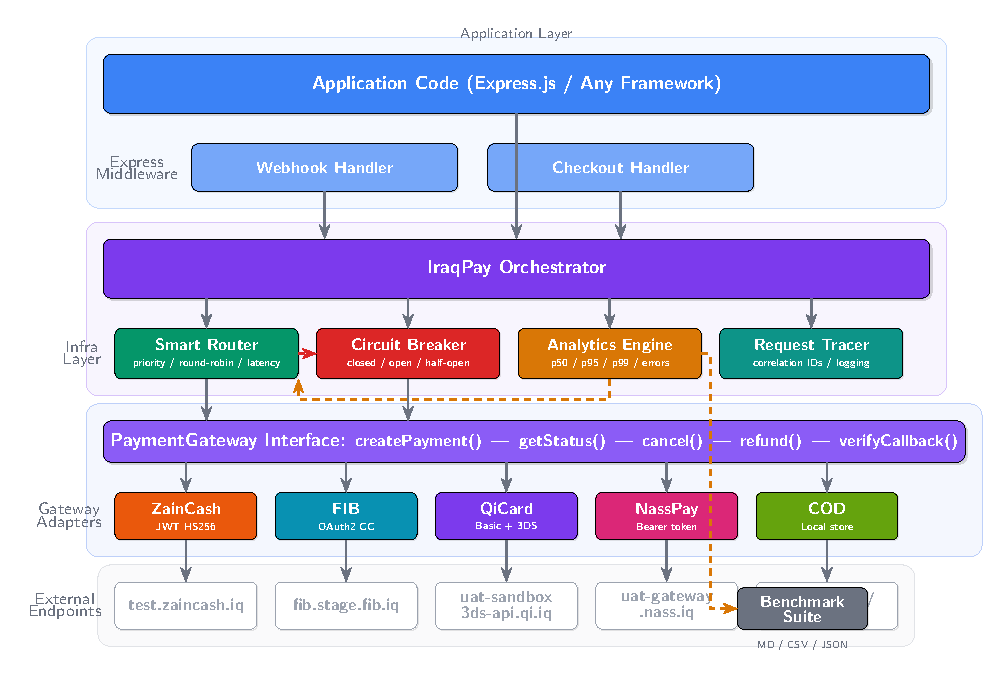
\includegraphics[width=\textwidth]{architecture.pdf}
\caption{IraqPay architecture. The \texttt{IraqPay} orchestrator delegates payment operations through the smart router and circuit breaker to gateway adapters, while the analytics engine and tracer record all operations.}
\label{fig:architecture}
\end{figure}

The core abstraction is the \texttt{PaymentGateway} interface, which every gateway adapter must implement:

\begin{lstlisting}[style=typescript,caption={Core gateway interface},label={lst:interface}]
interface PaymentGateway {
  readonly name: GatewayName;
  createPayment(params: CreatePaymentParams): Promise<PaymentResult>;
  getStatus(paymentId: string): Promise<PaymentStatusResult>;
  cancel(paymentId: string, amount?: number): Promise<boolean>;
  refund(paymentId: string, amount?: number): Promise<boolean>;
  verifyCallback(payload: unknown): Promise<WebhookEvent>;
}
\end{lstlisting}

Each gateway adapter encapsulates its specific authentication protocol, API endpoint construction, request/response mapping, and callback verification logic. The \texttt{IraqPay} orchestrator manages gateway lifecycle and delegates operations through three infrastructure layers:

\begin{enumerate}
\item \textbf{Smart Router:} Selects the optimal gateway based on configurable strategies (priority, round-robin, or lowest-latency) and provides automatic fallback chains when the primary gateway fails.
\item \textbf{Circuit Breaker:} Tracks per-gateway health using a three-state model (closed $\rightarrow$ open $\rightarrow$ half-open), automatically disabling failing gateways and periodically testing recovery.
\item \textbf{Analytics \& Tracing:} Records per-gateway latency distributions (p50, p95, p99), success/failure rates, error breakdowns, and attaches unique correlation IDs to every operation for end-to-end tracing.
\end{enumerate}

\subsection{Gateway Adapters}

Each adapter handles the full payment lifecycle within its gateway's constraints:

\textbf{ZainCash} uses JWT (HS256) for both request signing and callback verification. Payment parameters are encoded in a signed JWT and submitted to the ZainCash API, which returns a transaction ID. The user is redirected to complete payment, and the callback delivers a JWT token in a query parameter that the SDK verifies and decodes.

\textbf{FIB (First Iraqi Bank)} implements OAuth2 client credentials flow with automatic token refresh. Successful payment creation returns a QR code (base64), a human-readable code, and three mobile deep links (personal, business, corporate banking apps). The SDK handles 401 responses by transparently re-authenticating and retrying the request.

\textbf{QiCard} uses HTTP Basic authentication with an additional \texttt{X-Terminal-Id} header. Payments follow a 3D Secure redirect flow. The SDK always performs server-side status verification on callback receipt---a security best practice that prevents client-side tampering with redirect parameters.

\textbf{NassPay} authenticates via a login endpoint that returns a Bearer token with a time-to-live. The SDK implements conservative token caching with a 50-minute TTL (refreshing 10 minutes before expiry) and automatic retry on 401 responses.

\textbf{COD (Cash-on-Delivery)} is implemented as a local state tracker with a pluggable storage interface, allowing developers to substitute in-memory storage with a database adapter for production persistence.

\subsection{Circuit Breaker}

The circuit breaker implements the standard three-state pattern with per-gateway isolation:

\begin{itemize}
\item \textbf{Closed} (normal): Requests pass through. Consecutive failures are counted.
\item \textbf{Open} (failing): Requests are immediately rejected with a \texttt{CIRCUIT\_OPEN} error. After a configurable reset timeout (default: 30s), the circuit transitions to half-open.
\item \textbf{Half-open} (testing): A limited number of test requests are allowed through. If they succeed, the circuit closes; if any fail, it reopens.
\end{itemize}

Configuration supports per-gateway overrides, allowing different failure thresholds for gateways with known reliability differences.

\subsection{Smart Router}

The smart router supports three strategies:

\begin{enumerate}
\item \textbf{Priority:} Each gateway is assigned a numerical priority; the lowest value is selected first. This is the simplest strategy and suitable when one gateway is preferred.
\item \textbf{Round-robin:} Gateways are cycled in order, distributing load evenly. Useful for A/B testing or load balancing.
\item \textbf{Lowest-latency:} The gateway with the lowest median (p50) latency from the analytics engine is selected. This requires the analytics module and adapts dynamically to gateway performance changes.
\end{enumerate}

All strategies respect gateway rules (minimum/maximum amounts, supported currencies) and circuit breaker state. When the primary gateway fails, the router provides a fallback chain of alternative gateways.

\subsection{Analytics and Tracing}

The analytics engine collects metrics in a sliding window (configurable, default 1000 samples per gateway) and exposes aggregate and per-gateway views:

\begin{itemize}
\item Latency percentiles: p50, p95, p99, min, max, average
\item Success and failure counts with success rate
\item Error breakdown by error code
\item Event listeners for real-time monitoring
\end{itemize}

The tracing module assigns unique 128-bit correlation IDs to every payment operation. A structured \texttt{Logger} interface allows integration with any logging framework (Winston, Pino, Bunyan, or custom implementations). Log entries include trace ID, span ID, gateway name, operation type, duration, and optional metadata.

\subsection{Benchmark Suite}

The benchmark runner executes $N$ payment iterations per gateway and produces structured reports with:

\begin{itemize}
\item Per-gateway latency statistics (min, max, average, median, p95, p99, standard deviation)
\item Success rates and error distributions
\item Comparison tables
\item Export to Markdown (for documentation), CSV (for statistical analysis), and JSON (for programmatic consumption)
\end{itemize}

%% ════════════════════════════════════════════════════════════════════════════
\section{Illustrative Examples}
\label{sec:examples}
%% ════════════════════════════════════════════════════════════════════════════

\subsection{Basic Usage}

The simplest integration requires configuring at least one gateway:

\begin{lstlisting}[style=typescript,caption={Basic payment creation},label={lst:basic}]
import { IraqPay } from 'iraqpay';

const pay = new IraqPay({
  gateways: {
    zaincash: { msisdn: '...', merchantId: '...', secret: '...' },
    fib: { clientId: '...', clientSecret: '...' },
  },
  sandbox: true,
});

const payment = await pay.createPayment({
  gateway: 'zaincash',
  amount: 25000,
  orderId: 'order_123',
  callbackUrl: 'https://myapp.com/callback',
});

// ZainCash returns a redirect URL
console.log(payment.redirectUrl);

// FIB would return a QR code instead
// console.log(payment.qrCode);
\end{lstlisting}

\subsection{Smart Routing with Fallback}

When multiple gateways are configured, the smart router can automatically select the best gateway and fall back on failure:

\begin{lstlisting}[style=typescript,caption={Smart routing with circuit breaker and analytics},label={lst:routing}]
const pay = new IraqPay({
  gateways: {
    zaincash: { msisdn: '...', merchantId: '...', secret: '...' },
    fib: { clientId: '...', clientSecret: '...' },
    qicard: { username: '...', password: '...', terminalId: '...' },
  },
  router: {
    enabled: true,
    strategy: 'lowest-latency',
    fallbackChain: ['fib', 'zaincash', 'qicard'],
    rules: {
      zaincash: { minAmount: 250, currencies: ['IQD'] },
      fib: { currencies: ['IQD', 'USD'] },
    },
  },
  circuitBreaker: { failureThreshold: 3, resetTimeoutMs: 30000 },
  analytics: { enabled: true },
});

// No gateway specified --- router selects automatically
const payment = await pay.createPayment({
  amount: 10000,
  orderId: 'order_456',
  callbackUrl: 'https://myapp.com/webhook',
});
\end{lstlisting}

\subsection{Production Monitoring}

The analytics engine provides real-time gateway health monitoring:

\begin{lstlisting}[style=typescript,caption={Accessing per-gateway metrics},label={lst:metrics}]
// After processing payments...
const metrics = pay.analytics.getMetrics();

for (const [gw, m] of Object.entries(metrics.byGateway)) {
  console.log(`${gw}: ${m.successRate*100}% success, ` +
    `p50=${m.p50Ms}ms, p95=${m.p95Ms}ms`);
}

// Real-time event listener
pay.analytics.on((event) => {
  if (!event.success) {
    alertOps(`${event.gateway} failed: ${event.error?.message}`);
  }
});

// Circuit breaker status
const status = pay.circuitBreaker.getAllStatus();
console.log(status.filter(s => s.state !== 'closed'));
\end{lstlisting}

\subsection{Benchmarking}

The benchmark suite enables systematic performance comparison:

\begin{lstlisting}[style=typescript,caption={Running gateway benchmarks},label={lst:benchmark}]
import { BenchmarkRunner } from 'iraqpay';

const runner = new BenchmarkRunner(pay);
const report = await runner.run({
  iterations: 50,
  delayMs: 1000,
  gateways: ['zaincash', 'fib', 'qicard'],
});

// Markdown table for documentation
console.log(BenchmarkRunner.toMarkdown(report));

// CSV for statistical analysis
fs.writeFileSync('results.csv', BenchmarkRunner.toCsv(report));
\end{lstlisting}

%% ════════════════════════════════════════════════════════════════════════════
\section{Benchmark Results}
\label{sec:benchmarks}
%% ════════════════════════════════════════════════════════════════════════════

To demonstrate the benchmark suite and characterize gateway performance, we executed 50 payment creation requests against the ZainCash sandbox and COD gateway, and 10 network reachability probes against FIB, QiCard, and NassPay sandbox endpoints. Table~\ref{tab:benchmark-results} summarizes the results.

\begin{table}[!t]
\centering
\caption{Gateway benchmark results (sandbox mode, March 2026)}
\label{tab:benchmark-results}
\small
\begin{tabular}{@{}lrrrrrrrr@{}}
\toprule
\textbf{Gateway} & \textbf{N} & \textbf{Success\%} & \textbf{Avg (ms)} & \textbf{Med (ms)} & \textbf{P95 (ms)} & \textbf{P99 (ms)} & \textbf{Min (ms)} & \textbf{StdDev} \\
\midrule
ZainCash & 50 & 100\% & 279 & 248 & 391 & 934 & 229 & 113 \\
COD      & 50 & 100\% & $<$1 & $<$1 & $<$1 & $<$1 & 0 & $<$1 \\
\midrule
\multicolumn{9}{l}{\textit{Network reachability probes (auth fails, measures endpoint RTT):}} \\
FIB$^\dagger$      & 10 & 0\% & 137 & 188 & --- & --- & --- & --- \\
QiCard$^\dagger$   & 10 & 0\% & 150 & 171 & --- & --- & --- & --- \\
NassPay$^\dagger$  & 10 & 0\% & 127 & 167 & --- & --- & --- & --- \\
\bottomrule
\end{tabular}
\vspace{4pt}
\raggedright\small $^\dagger$FIB, QiCard, and NassPay sandbox endpoints require merchant registration for valid credentials. Probe latencies reflect network round-trip time to first HTTP error response (401/403/422), confirming endpoint availability. COD is local-only with no network I/O. All benchmarks executed from Najaf, Iraq.
\end{table}

ZainCash exhibits stable performance with a median latency of 248~ms and 100\% success rate over 50 consecutive requests. The first request shows a cold-start penalty (934~ms), after which latency stabilizes in the 229--355~ms range. The COD gateway, being purely local, operates at sub-millisecond latency. Network probes to FIB, QiCard, and NassPay confirm that all sandbox endpoints are reachable from Iraq with round-trip times of 127--188~ms, consistent with regional hosting.

%% ════════════════════════════════════════════════════════════════════════════
\section{Case Study: Akel Bait Food Marketplace}
\label{sec:casestudy}
%% ════════════════════════════════════════════════════════════════════════════

IraqPay is deployed in \emph{Akel Bait}, a production food marketplace serving customers in Iraqi cities. The application uses IraqPay to offer ZainCash mobile payments alongside cash-on-delivery, with the smart router configured to fall back to COD when ZainCash is unavailable.

The integration required fewer than 20 lines of application code---a single \texttt{IraqPay} instantiation and a \texttt{createPayment} call in the checkout flow. The Express.js webhook middleware handles all callback verification and status updates automatically. The analytics engine provides the operations team with real-time visibility into payment success rates and gateway latency, enabling data-driven decisions about which gateways to prioritize.

%% ════════════════════════════════════════════════════════════════════════════
\section{Impact and Generalizability}
\label{sec:impact}
%% ════════════════════════════════════════════════════════════════════════════

While IraqPay targets the Iraqi market, its architecture is intentionally general. The adapter pattern, circuit breaker, smart router, and analytics engine are gateway-agnostic---adding a new gateway requires only implementing the \texttt{PaymentGateway} interface (five methods). This makes the pattern directly applicable to other fragmented payment ecosystems, such as:

\begin{itemize}
\item \textbf{Bangladesh} (bKash, Nagad, Rocket, SSLCommerz)
\item \textbf{Pakistan} (JazzCash, EasyPaisa, HBL, UBL)
\item \textbf{Nigeria} (Paystack, Flutterwave, Interswitch, Remita)
\item \textbf{Egypt} (Fawry, Paymob, Accept, Aman)
\end{itemize}

The open-source availability (MIT license) and npm distribution model lower the barrier for developers in these markets to either adopt IraqPay directly or fork it as a starting point.

%% ════════════════════════════════════════════════════════════════════════════
\section{Conclusions}
\label{sec:conclusions}
%% ════════════════════════════════════════════════════════════════════════════

IraqPay demonstrates that payment gateway fragmentation in emerging markets can be effectively addressed through a well-designed adapter-pattern SDK with production-grade infrastructure. The key contributions are:

\begin{enumerate}
\item The first open-source unified SDK for Iraqi payment gateways, abstracting five heterogeneous APIs behind a single interface.
\item Production infrastructure (circuit breaker, smart router, analytics, tracing) that goes beyond simple API unification to address real-world reliability and observability requirements.
\item A benchmark suite that enables systematic, reproducible gateway performance comparison---a tool currently absent from the fintech ecosystem.
\item An architecture pattern that generalizes to any fragmented payment ecosystem, with new gateways requiring only a single interface implementation.
\end{enumerate}

The software is published on npm (\texttt{npm install iraqpay}), available on GitHub under the MIT license, and deployed in a production food marketplace. Future work includes adding support for subscription/recurring payments, integrating with additional Middle Eastern gateways, and conducting a longitudinal study of gateway reliability in production.

%% ════════════════════════════════════════════════════════════════════════════
%% References
%% ════════════════════════════════════════════════════════════════════════════

\begin{thebibliography}{10}

\bibitem{gamma1994design}
E.~Gamma, R.~Helm, R.~Johnson, and J.~Vlissides,
\newblock {\em Design Patterns: Elements of Reusable Object-Oriented Software},
\newblock Addison-Wesley, 1994.

\bibitem{nygard2018release}
M.~T. Nygard,
\newblock {\em Release It!: Design and Deploy Production-Ready Software},
\newblock Pragmatic Bookshelf, 2nd edition, 2018.

\bibitem{fowler2014circuitbreaker}
M.~Fowler,
\newblock Circuit Breaker,
\newblock \url{https://martinfowler.com/bliki/CircuitBreaker.html}, 2014.

\bibitem{stripe2023docs}
Stripe, Inc.,
\newblock Stripe API Reference,
\newblock \url{https://stripe.com/docs/api}, 2023.

\bibitem{worldbank2023iraq}
World Bank,
\newblock Iraq Economic Monitor: Navigating Uncertainty,
\newblock World Bank Group, Washington, D.C., 2023.

\bibitem{gsma2023mobile}
GSMA,
\newblock State of the Industry Report on Mobile Money 2023,
\newblock GSMA, London, 2023.

\bibitem{zaincash2024api}
Zain Cash,
\newblock ZainCash API Documentation,
\newblock \url{https://docs.zaincash.iq}, 2024.

\bibitem{fib2024api}
First Iraqi Bank,
\newblock FIB Payment Gateway Developer Guide,
\newblock \url{https://fib.iq}, 2024.

\end{thebibliography}

\end{document}
